% Options for packages loaded elsewhere
\PassOptionsToPackage{unicode}{hyperref}
\PassOptionsToPackage{hyphens}{url}
\PassOptionsToPackage{dvipsnames,svgnames,x11names}{xcolor}
%
\documentclass[
  letterpaper,
  DIV=11,
  numbers=noendperiod]{scrartcl}

\usepackage{amsmath,amssymb}
\usepackage{iftex}
\ifPDFTeX
  \usepackage[T1]{fontenc}
  \usepackage[utf8]{inputenc}
  \usepackage{textcomp} % provide euro and other symbols
\else % if luatex or xetex
  \usepackage{unicode-math}
  \defaultfontfeatures{Scale=MatchLowercase}
  \defaultfontfeatures[\rmfamily]{Ligatures=TeX,Scale=1}
\fi
\usepackage{lmodern}
\ifPDFTeX\else  
    % xetex/luatex font selection
\fi
% Use upquote if available, for straight quotes in verbatim environments
\IfFileExists{upquote.sty}{\usepackage{upquote}}{}
\IfFileExists{microtype.sty}{% use microtype if available
  \usepackage[]{microtype}
  \UseMicrotypeSet[protrusion]{basicmath} % disable protrusion for tt fonts
}{}
\makeatletter
\@ifundefined{KOMAClassName}{% if non-KOMA class
  \IfFileExists{parskip.sty}{%
    \usepackage{parskip}
  }{% else
    \setlength{\parindent}{0pt}
    \setlength{\parskip}{6pt plus 2pt minus 1pt}}
}{% if KOMA class
  \KOMAoptions{parskip=half}}
\makeatother
\usepackage{xcolor}
\setlength{\emergencystretch}{3em} % prevent overfull lines
\setcounter{secnumdepth}{-\maxdimen} % remove section numbering
% Make \paragraph and \subparagraph free-standing
\makeatletter
\ifx\paragraph\undefined\else
  \let\oldparagraph\paragraph
  \renewcommand{\paragraph}{
    \@ifstar
      \xxxParagraphStar
      \xxxParagraphNoStar
  }
  \newcommand{\xxxParagraphStar}[1]{\oldparagraph*{#1}\mbox{}}
  \newcommand{\xxxParagraphNoStar}[1]{\oldparagraph{#1}\mbox{}}
\fi
\ifx\subparagraph\undefined\else
  \let\oldsubparagraph\subparagraph
  \renewcommand{\subparagraph}{
    \@ifstar
      \xxxSubParagraphStar
      \xxxSubParagraphNoStar
  }
  \newcommand{\xxxSubParagraphStar}[1]{\oldsubparagraph*{#1}\mbox{}}
  \newcommand{\xxxSubParagraphNoStar}[1]{\oldsubparagraph{#1}\mbox{}}
\fi
\makeatother


\providecommand{\tightlist}{%
  \setlength{\itemsep}{0pt}\setlength{\parskip}{0pt}}\usepackage{longtable,booktabs,array}
\usepackage{calc} % for calculating minipage widths
% Correct order of tables after \paragraph or \subparagraph
\usepackage{etoolbox}
\makeatletter
\patchcmd\longtable{\par}{\if@noskipsec\mbox{}\fi\par}{}{}
\makeatother
% Allow footnotes in longtable head/foot
\IfFileExists{footnotehyper.sty}{\usepackage{footnotehyper}}{\usepackage{footnote}}
\makesavenoteenv{longtable}
\usepackage{graphicx}
\makeatletter
\newsavebox\pandoc@box
\newcommand*\pandocbounded[1]{% scales image to fit in text height/width
  \sbox\pandoc@box{#1}%
  \Gscale@div\@tempa{\textheight}{\dimexpr\ht\pandoc@box+\dp\pandoc@box\relax}%
  \Gscale@div\@tempb{\linewidth}{\wd\pandoc@box}%
  \ifdim\@tempb\p@<\@tempa\p@\let\@tempa\@tempb\fi% select the smaller of both
  \ifdim\@tempa\p@<\p@\scalebox{\@tempa}{\usebox\pandoc@box}%
  \else\usebox{\pandoc@box}%
  \fi%
}
% Set default figure placement to htbp
\def\fps@figure{htbp}
\makeatother
% definitions for citeproc citations
\NewDocumentCommand\citeproctext{}{}
\NewDocumentCommand\citeproc{mm}{%
  \begingroup\def\citeproctext{#2}\cite{#1}\endgroup}
\makeatletter
 % allow citations to break across lines
 \let\@cite@ofmt\@firstofone
 % avoid brackets around text for \cite:
 \def\@biblabel#1{}
 \def\@cite#1#2{{#1\if@tempswa , #2\fi}}
\makeatother
\newlength{\cslhangindent}
\setlength{\cslhangindent}{1.5em}
\newlength{\csllabelwidth}
\setlength{\csllabelwidth}{3em}
\newenvironment{CSLReferences}[2] % #1 hanging-indent, #2 entry-spacing
 {\begin{list}{}{%
  \setlength{\itemindent}{0pt}
  \setlength{\leftmargin}{0pt}
  \setlength{\parsep}{0pt}
  % turn on hanging indent if param 1 is 1
  \ifodd #1
   \setlength{\leftmargin}{\cslhangindent}
   \setlength{\itemindent}{-1\cslhangindent}
  \fi
  % set entry spacing
  \setlength{\itemsep}{#2\baselineskip}}}
 {\end{list}}
\usepackage{calc}
\newcommand{\CSLBlock}[1]{\hfill\break\parbox[t]{\linewidth}{\strut\ignorespaces#1\strut}}
\newcommand{\CSLLeftMargin}[1]{\parbox[t]{\csllabelwidth}{\strut#1\strut}}
\newcommand{\CSLRightInline}[1]{\parbox[t]{\linewidth - \csllabelwidth}{\strut#1\strut}}
\newcommand{\CSLIndent}[1]{\hspace{\cslhangindent}#1}

\KOMAoption{captions}{tableheading}
\makeatletter
\@ifpackageloaded{caption}{}{\usepackage{caption}}
\AtBeginDocument{%
\ifdefined\contentsname
  \renewcommand*\contentsname{Table of contents}
\else
  \newcommand\contentsname{Table of contents}
\fi
\ifdefined\listfigurename
  \renewcommand*\listfigurename{List of Figures}
\else
  \newcommand\listfigurename{List of Figures}
\fi
\ifdefined\listtablename
  \renewcommand*\listtablename{List of Tables}
\else
  \newcommand\listtablename{List of Tables}
\fi
\ifdefined\figurename
  \renewcommand*\figurename{Figure}
\else
  \newcommand\figurename{Figure}
\fi
\ifdefined\tablename
  \renewcommand*\tablename{Table}
\else
  \newcommand\tablename{Table}
\fi
}
\@ifpackageloaded{float}{}{\usepackage{float}}
\floatstyle{ruled}
\@ifundefined{c@chapter}{\newfloat{codelisting}{h}{lop}}{\newfloat{codelisting}{h}{lop}[chapter]}
\floatname{codelisting}{Listing}
\newcommand*\listoflistings{\listof{codelisting}{List of Listings}}
\makeatother
\makeatletter
\makeatother
\makeatletter
\@ifpackageloaded{caption}{}{\usepackage{caption}}
\@ifpackageloaded{subcaption}{}{\usepackage{subcaption}}
\makeatother

\usepackage{bookmark}

\IfFileExists{xurl.sty}{\usepackage{xurl}}{} % add URL line breaks if available
\urlstyle{same} % disable monospaced font for URLs
\hypersetup{
  pdftitle={Research Report on the Clorox Company (CLX)},
  pdfkeywords={Financial Report, Feduciary},
  colorlinks=true,
  linkcolor={blue},
  filecolor={Maroon},
  citecolor={Blue},
  urlcolor={Blue},
  pdfcreator={LaTeX via pandoc}}


\title{Research Report on the Clorox Company (CLX)}
\author{Andrey Malyukov \and Roza Bass}
\date{}

\begin{document}
\maketitle
\begin{abstract}
In September 2021, a significant jump in seismic activity on the island
of La Palma (Canary Islands, Spain) signaled the start of a volcanic
crisis that still continues at the time of writing. Earthquake data is
continually collected and published by the Instituto Geográphico
Nacional (IGN). \ldots{}
\end{abstract}

\renewcommand*\contentsname{Table of contents}
{
\hypersetup{linkcolor=}
\setcounter{tocdepth}{3}
\tableofcontents
}

\subsection{TODO}\label{todo}

Use ``PerformanceAnalytics'' package for Sharpe ratio and risk analysis.

Cite your stuff: (Regenstein 2020).

\subsection{Introduction}\label{introduction}

\section{}\label{section}

\begin{quote}
\textbf{On the simplified nature of analysis in this document.}

Subject of financial analysis is very information-dense and to perform
such an analysis (be it an analysis of industrial sectors, fundamental,
technical, etc.) in earnest is a non-trivial job that we don't see
ourselves capable of performing.

Therefore, this document aims to provide a simplified, non-rigorous
analysis aiming to showcase our understanding of course material and
minimal proficiency in scientific communication using tools such as R
language {``R: {The R Project} for {Statistical Computing}''} (n.d.),
its ``tidyquant'' package Dancho and Vaughan (2025) and Quarto
scientific publishing system {``Quarto''} (n.d.).
\end{quote}

\pandocbounded{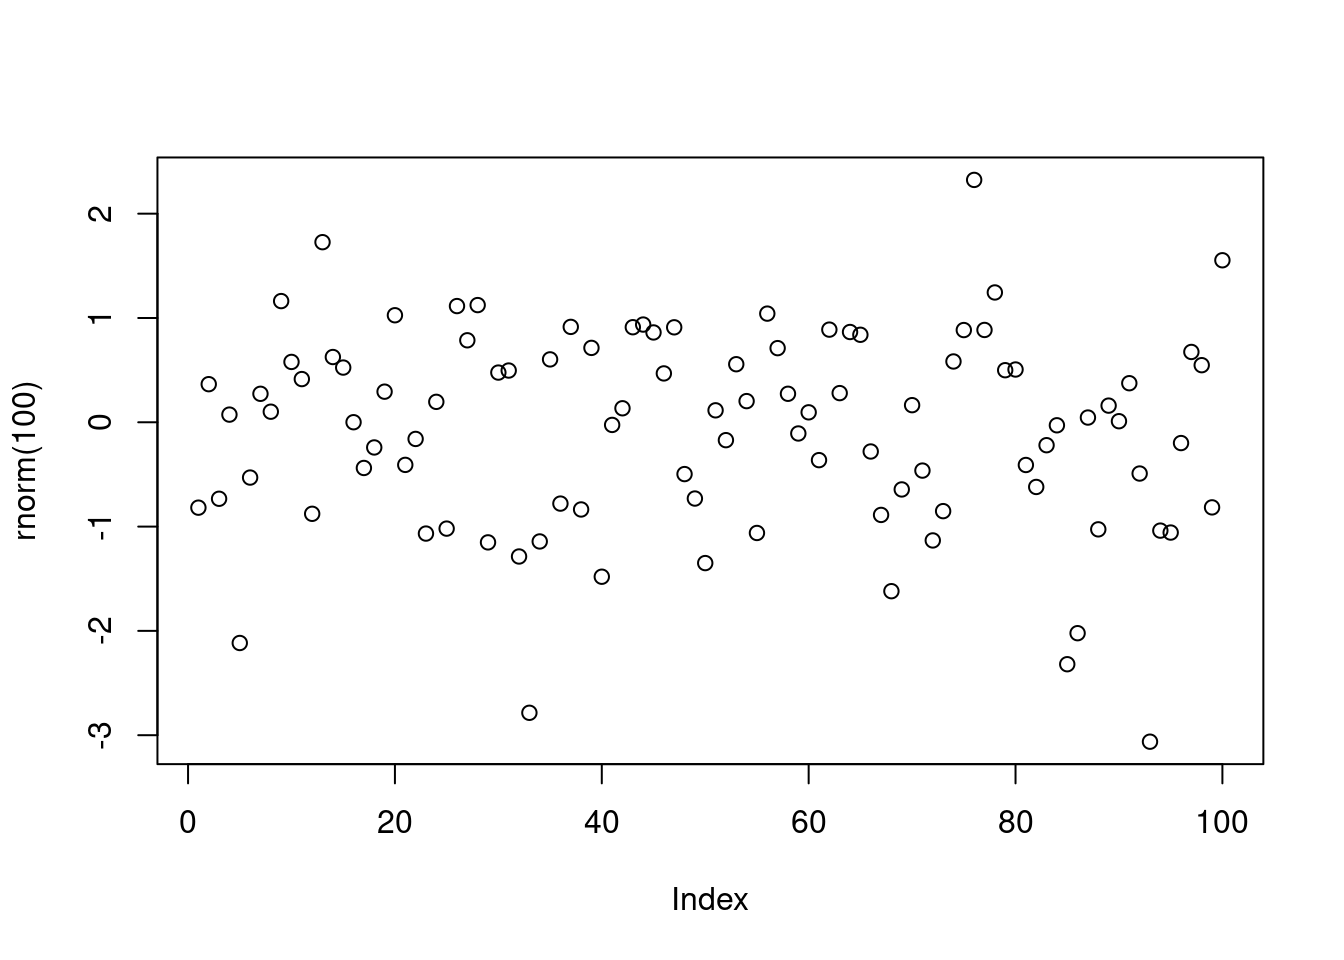
\includegraphics[keepaspectratio]{index_files/figure-latex/notebooks-intro-cell-2-output-1.png}}

We need better stuff though.

\begin{verbatim}
[1] "CPALTT01USQ657N"           CPALTT01USQ657N
1955-04-01       0.0000000
1955-07-01       0.4993758
1955-10-01       0.1242236
1956-01-01      -0.2481390
1956-04-01       0.8706468
1956-07-01       1.2330456     Index            CPALTT01USQ657N  
 Min.   :1955-04-01   Min.   :-2.8285  
 1st Qu.:1972-06-08   1st Qu.: 0.3950  
 Median :1989-08-16   Median : 0.8018  
 Mean   :1989-08-16   Mean   : 0.8959  
 3rd Qu.:2006-10-24   3rd Qu.: 1.1939  
 Max.   :2024-01-01   Max.   : 3.9508  
\end{verbatim}

\begin{table}

\caption{\label{tbl-planets}Astronomical object}

\centering{

\subcaption{\label{tbl-planets-1}}

\centering{

\pandocbounded{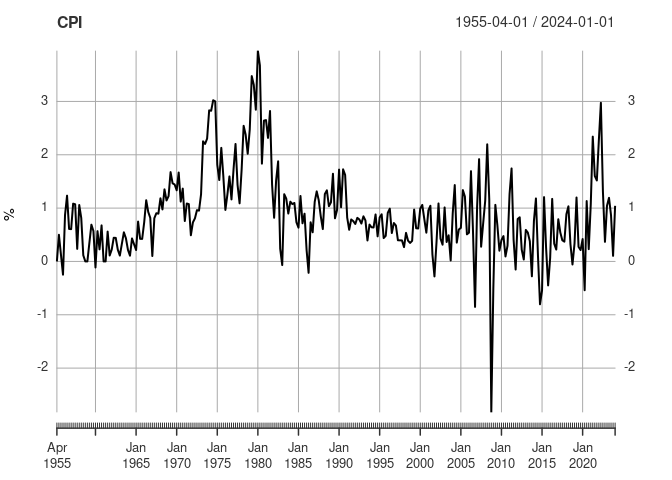
\includegraphics[keepaspectratio]{index_files/figure-latex/notebooks-intro-tbl-planets-output-3.png}}

}

}

\end{table}%

Use this kind of macroeconomic analysis maybe?

\subsection{Sector Analysis}\label{sector-analysis}

Performance of all sectors relative to each other.

https://alphaarchitect.com/2020/01/visualization-sector-trends-with-r-code/

Maybe that's a bit much.

\section{}\label{section-1}

\subsubsection{Financial Analysis of The Clorox Company (CLX) in the
Consumer Defensive
Sector}\label{financial-analysis-of-the-clorox-company-clx-in-the-consumer-defensive-sector}

\paragraph{\texorpdfstring{\textbf{1. Sector
Analysis}}{1. Sector Analysis}}\label{sector-analysis-1}

Clorox operates in the \textbf{Consumer Defensive sector}, specifically
within the Household and Personal Products sub-sector. This sector is
characterized by stable demand and recession resilience.

Sector's \textbf{Market Cap} is estimated to be \$3.7 trillion. The
\textbf{Market weight (share)} of the sector relative to the other 10
sectors is 5.45\%.

Sector's \textbf{Year-To-Date Return} is 6.17\%, which outperforms
S\&P500 (3.54\%).

\begin{center}\rule{0.5\linewidth}{0.5pt}\end{center}

\paragraph{\texorpdfstring{\textbf{2. Position Relative to
Competitors}}{2. Position Relative to Competitors}}\label{position-relative-to-competitors}

Clorox's market share inside it's sector is relatively small:

\begin{longtable}[]{@{}
  >{\raggedright\arraybackslash}p{(\linewidth - 8\tabcolsep) * \real{0.2192}}
  >{\raggedright\arraybackslash}p{(\linewidth - 8\tabcolsep) * \real{0.2329}}
  >{\raggedright\arraybackslash}p{(\linewidth - 8\tabcolsep) * \real{0.2329}}
  >{\raggedright\arraybackslash}p{(\linewidth - 8\tabcolsep) * \real{0.1644}}
  >{\raggedright\arraybackslash}p{(\linewidth - 8\tabcolsep) * \real{0.1507}}@{}}
\toprule\noalign{}
\begin{minipage}[b]{\linewidth}\raggedright
COMPANY NAME
\end{minipage} & \begin{minipage}[b]{\linewidth}\raggedright
MARKET SHARE 12 Months Ending Q4 2024
\end{minipage} & \begin{minipage}[b]{\linewidth}\raggedright
MARKET SHARE 12 Months Ending Q3 2024
\end{minipage} & \begin{minipage}[b]{\linewidth}\raggedright
MARKET SHARE MRQ Q4 2024
\end{minipage} & \begin{minipage}[b]{\linewidth}\raggedright
MARKET SHARE Q3 2024
\end{minipage} \\
\midrule\noalign{}
\endhead
\bottomrule\noalign{}
\endlastfoot
\textbf{The Clorox Company} & 2.61\% & 2.80\% & 2.42 \% & 2.66 \% \\
The Campbells Company & 3.60\% & 3.61\% & 3.97\% & 3.46\% \\
Colgate palmolive Company & 7.32\% & 7.54\% & 7.09\% & 7.59\% \\
Conagra Brands Inc & 4.58\% & 4.61\% & 4.58\% & 4.21\% \\
Ecolab Inc & 5.06\% & 5.07\% & 5.26\% & 5.40\% \\
Mccormick and Company Incorporated & 2.45\% & 2.50\% & 2.58\% &
2.53\% \\
Procter and Gamble Co & 30.72\% & 31.46\% & 31.37\% & 32.77\% \\
Hormel Foods Corporation & 5.52\% & 5.65\% & 5.09\% & 4.37\% \\
Avon Products Inc & 1.15\% & 1.28\% & 0.95\% & 1.23\% \\
Horizon Kinetics Holding Corporation & 0.01\% & 0.00\% & 0.02\% &
0.00\% \\
Ingredion Incorporated & 2.75\% & 2.89\% & 2.68\% & 2.83\% \\
Lancaster Colony Corporation & 0.69\% & 0.70\% & 0.73\% & 0.70\% \\
J and j Snack Foods Corp & 0.58\% & 0.59\% & 0.52\% & 0.64\% \\
Treehouse Foods Inc & 1.19\% & 1.24\% & 1.20\% & 1.19\% \\
Dole Plc & 3.00\% & 3.46\% & 3.00\% & 3.46\% \\
Church and Dwight Co Inc & 2.22\% & 2.27\% & 2.27\% & 2.28\% \\
Coty Inc & 2.22\% & 2.30\% & 2.39\% & 2.52\% \\
Unilever Plc & 24.32\% & 22.02\% & 24.32\% & 22.02\% \\
SUBTOTAL & 100\% & 100\% & 100\% & 100\% \\
\end{longtable}

CLX's Market share relative to its competitors, as of Q4 2024 within the
Consumer Non Cyclical Sector (i.e.~Consumer Defensive), source: {``The
{Clorox Market} Share Relative to Its Competitors, as of {Q4} 2024 -
{CSIMarket}''} (n.d.)

Clorox competes with major players such as \textbf{Procter \& Gamble
(PG)}, \textbf{Colgate-Palmolive (CL)}, \textbf{Church \& Dwight (CHD)},
and \textbf{Kimberly-Clark (KMB)}.

\pandocbounded{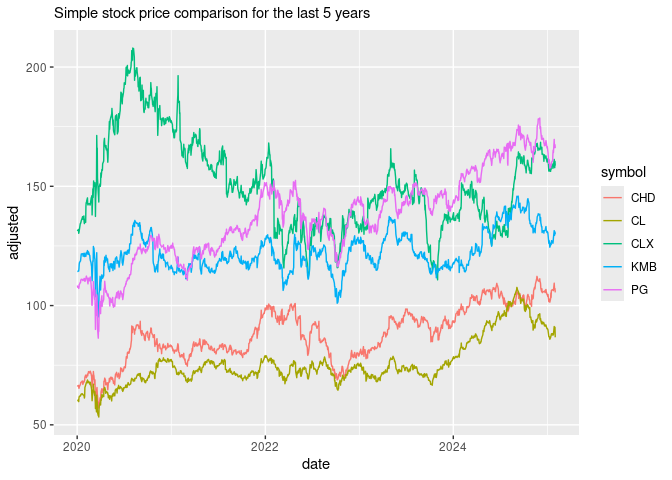
\includegraphics[keepaspectratio]{index_files/figure-latex/notebooks-sector-cell-2-output-2.png}}

\begin{center}\rule{0.5\linewidth}{0.5pt}\end{center}

\begin{center}\rule{0.5\linewidth}{0.5pt}\end{center}

\paragraph{\texorpdfstring{\textbf{4. Strategic and Financial
Challenges}}{4. Strategic and Financial Challenges}}\label{strategic-and-financial-challenges}

\begin{itemize}
\tightlist
\item
  \textbf{Cyberattack Impact}: Caused a 20\% Q1 FY24 sales decline,
  though recovery efforts restored \textasciitilde90\% market share by
  Q3 .
\item
  \textbf{Margin Recovery}: Gross margin expanded to 46.5\% in Q4 FY24,
  driven by cost savings .
\item
  \textbf{Divestitures}: Sold non-core businesses (Argentina, VMS) to
  focus on high-growth segments .
\end{itemize}

\begin{center}\rule{0.5\linewidth}{0.5pt}\end{center}

\begin{center}\rule{0.5\linewidth}{0.5pt}\end{center}

\paragraph{\texorpdfstring{\textbf{6. Key
Insights}}{6. Key Insights}}\label{key-insights}

\begin{itemize}
\tightlist
\item
  Clorox's valuation (P/E 40.6) reflects optimism about its recovery and
  IGNITE strategy but is expensive compared to peers .
\item
  Consumer Staples sector growth (CAGR 3.7\% for cleaning products)
  supports long-term stability, but competition from eco-friendly brands
  (e.g., Seventh Generation) poses risks .
\item
  Clorox's underperformance vs.~indices highlights sector-specific
  challenges (inflation, supply chain) .
\end{itemize}

\begin{center}\rule{0.5\linewidth}{0.5pt}\end{center}

For real-time data, update the R code with current ticker prices and
adjust the date range. The analysis underscores Clorox's resilience in a
defensive sector but signals caution due to margin pressures and
competitive headwinds.

\subsection{Personality of the
Company}\label{personality-of-the-company}

\section{}\label{section-2}

\paragraph{\texorpdfstring{\textbf{1. Company Purpose and
Responsibility}}{1. Company Purpose and Responsibility}}\label{company-purpose-and-responsibility}

\subparagraph{\texorpdfstring{\textbf{1. Company
Purpose}}{1. Company Purpose}}\label{company-purpose}

Clorox's stated purpose is to ``champion people to be well and thrive
every single day'' {``Purpose \& {Values}''} (n.d.). As a health and
wellness company, Clorox aims to make a meaningful and positive impact
on the world by improving the health and safety of employees, consumers,
and communities. All of this is reflected in their family-friendly and
inclusive branding.

\subparagraph{\texorpdfstring{\textbf{2. Responsibility
Policies}}{2. Responsibility Policies}}\label{responsibility-policies}

Clorox integrates environmental, social, and governance (ESG) goals into
its core business strategy {``Responsibility''} (n.d.). Key areas of
focus include:

\begin{itemize}
\tightlist
\item
  \textbf{Healthy Lives}: Promoting employee well-being, product
  stewardship, and transparency in ingredients.\\
\item
  \textbf{Clean World}: Reducing greenhouse gas emissions, plastic
  waste, and transitioning to 100\% renewable energy in U.S. and Canada
  operations.\\
\item
  \textbf{Thriving Communities}: Ensuring pay equity, fostering
  diversity, and supporting community initiatives.
\end{itemize}

Clorox has set ambitious targets, such as achieving net-zero emissions
by 2050.

\subparagraph{\texorpdfstring{\textbf{3. IGNITE
Strategy}}{3. IGNITE Strategy}}\label{ignite-strategy}

The IGNITE strategy is Clorox's long-term plan to drive what the company
calls a ``purpose-driven growth'' {``{IGNITE Strategy}''} (n.d.) by
aligning financial goals with ESG priorities. Key pillars include:

\begin{itemize}
\tightlist
\item
  \textbf{Fuel Growth}: Leveraging technology and sustainability to
  generate cost savings and reinvest in brands.\\
\item
  \textbf{Innovate Experiences}: Building purpose-driven brands and
  enhancing consumer experiences through personalized and sustainable
  products.\\
\item
  \textbf{Reimagine Work}: Creating an inclusive workplace and
  simplifying operations to drive efficiency.\\
\item
  \textbf{Evolve Portfolio}: Expanding into consumer megatrends like
  sustainability and wellness.
\end{itemize}

The strategy also includes specific financial targets, such as 2-4\% net
sales growth and 11-13\% free cash flow generation.

\paragraph{\texorpdfstring{\textbf{2. Key Executives, Their Commitment
and
Performance}}{2. Key Executives, Their Commitment and Performance}}\label{key-executives-their-commitment-and-performance}

\begin{longtable}[]{@{}
  >{\raggedright\arraybackslash}p{(\linewidth - 6\tabcolsep) * \real{0.2432}}
  >{\raggedright\arraybackslash}p{(\linewidth - 6\tabcolsep) * \real{0.5405}}
  >{\raggedright\arraybackslash}p{(\linewidth - 6\tabcolsep) * \real{0.0946}}
  >{\raggedright\arraybackslash}p{(\linewidth - 6\tabcolsep) * \real{0.1216}}@{}}
\toprule\noalign{}
\begin{minipage}[b]{\linewidth}\raggedright
Name
\end{minipage} & \begin{minipage}[b]{\linewidth}\raggedright
Title
\end{minipage} & \begin{minipage}[b]{\linewidth}\raggedright
Pay
\end{minipage} & \begin{minipage}[b]{\linewidth}\raggedright
Year Born
\end{minipage} \\
\midrule\noalign{}
\endhead
\bottomrule\noalign{}
\endlastfoot
Ms.~Linda J. Rendle & CEO \& Chairman & 3.93M & 1979 \\
Mr.~Kevin B. Jacobsen & Executive VP \& CFO & 1.91M & 1967 \\
Mr.~Eric H. Reynolds & Executive VP and Chief Operating \& Strategy
Officer & 1.96M & 1970 \\
Ms.~Angela C. Hilt & Executive VP, Chief Legal Officer \& Corporate
Secretary & 1.45M & 1972 \\
Ms.~Kirsten M. Marriner & Executive VP and Chief People \& Corporate
Affairs Officer & 1.54M & 1973 \\
Ms.~Laura E. Peck & VP, Chief Accounting Officer \& Corporate Controller
& -- & 1977 \\
Ms.~Chau Banks & Senior VP and Chief Information \& Data Officer & -- &
1970 \\
Ms.~Lisah Burhan & Vice President of Investor Relations & -- & -- \\
Mr.~Eric Sean Schwartz & Senior VP \& Chief Marketing Officer & -- &
1972 \\
Mr.~Erbie L. Foster Jr. & Chief Diversity Officer & -- & -- \\
\end{longtable}

Key Executives, source: {``The {Clorox Company} ({CLX}) {Company
Profile} \& {Facts}''} (n.d.)

According to {``The {Clorox Company}: {Business Model}, {SWOT Analysis},
and {Competitors} 2024 - {PitchGrade}''} (n.d.), CEO and Chairman Linda
J. Rendle, as well as the other executives and board members have
significant ownership stakes at the company, indicating high confidence
in their business.

Financial analysis website Simply WallSt gives the upper management team
at Clorox high marks on all 4 criteria: Compensation vs Market,
Compensation vs Earnings, Experienced Management and Experienced Board
{``The {Clorox Company} ({CLX}) {Leadership} \& {Management Team
Analysis}''} (n.d.).

\paragraph{\texorpdfstring{\textbf{3. Company Brand and
Reputation}}{3. Company Brand and Reputation}}\label{company-brand-and-reputation}

Clorox is a globally recognized leader in the cleaning and consumer
products industry, known for its trusted brands such as \textbf{Clorox
Bleach}, \textbf{Pine-Sol}, \textbf{Hidden Valley}, \textbf{Brita}, and
\textbf{Burt's Bees}.

The company has received numerous accolades, including being named one
of \textbf{America's Greenest Companies} by Newsweek, a \textbf{Safer
Choice Partner of the Year} by the EPA, and a top performer in the
\textbf{Human Rights Campaign Foundation's Corporate Equality Index}.
Its sustainable brands, such as \textbf{Brita}, \textbf{Burt's Bees},
and \textbf{Green Works}, have gained significant consumer trust for
their eco-friendly and socially responsible practices {``Recognitions''}
(n.d.).

\begin{center}\rule{0.5\linewidth}{0.5pt}\end{center}

In August 2023, Clorox experienced a severe \textbf{cyberattack}
Mascellino (2023) that disrupted its IT systems and operations. The
attack, which was detected on August 14, forced the company to take
affected systems offline, leading to significant production delays and
supply chain disruptions. Clorox activated its business continuity
plans, reverting to manual processes for order fulfillment and customer
communications.

The cyberattack had a material financial impact, with Clorox reporting a
23-28\% decline in quarterly sales and a drop in its stock price by over
25\% following the incident.

Clorox's response to the cyberattack highlighted its crisis management
capabilities. The company maintained transparency by providing regular
updates to stakeholders and implementing phased recovery plans to
restore operations safely. Brand and reputation were not severely
damaged in the process.

\subsection{Fundamental Analysis}\label{fundamental-analysis}

\section{}\label{section-3}

\subsubsection{Fundamental Analysis of The Clorox Company
(CLX)}\label{fundamental-analysis-of-the-clorox-company-clx}

Incorporating \textbf{Graham Number} and key financial ratios derived
from the latest available data (as of February 2025):

\begin{center}\rule{0.5\linewidth}{0.5pt}\end{center}

\paragraph{\texorpdfstring{\textbf{I. Graham Number
Calculation}}{I. Graham Number Calculation}}\label{i.-graham-number-calculation}

The Graham Number estimates a stock's intrinsic value using earnings per
share (EPS) and book value per share (BVPS):\\
\textbf{Formula}:

\(\text{Graham Number} = \sqrt{22.5 \times \text{EPS} \times \text{BVPS}}\)

\begin{itemize}
\tightlist
\item
  \textbf{EPS (TTM)}: \$3.67\\
\item
  \textbf{BVPS}: \$0.98 (Total Equity: \$121M / Shares Outstanding:
  123.19M)\\
\item
  \textbf{Calculation}:\\
  \(\sqrt{22.5 \times 3.67 \times 0.98} = \sqrt{80.92} \approx \boxed{8.99}\)
\item
  \textbf{Interpretation}: CLX's current stock price
  (\textasciitilde\$149.61) far exceeds the Graham Number, indicating
  potential overvaluation based on traditional metrics .
\end{itemize}

\begin{center}\rule{0.5\linewidth}{0.5pt}\end{center}

\paragraph{\texorpdfstring{\textbf{II. Key Financial
Ratios}}{II. Key Financial Ratios}}\label{ii.-key-financial-ratios}

\begin{longtable}[]{@{}
  >{\raggedright\arraybackslash}p{(\linewidth - 8\tabcolsep) * \real{0.0959}}
  >{\raggedright\arraybackslash}p{(\linewidth - 8\tabcolsep) * \real{0.1233}}
  >{\raggedright\arraybackslash}p{(\linewidth - 8\tabcolsep) * \real{0.1370}}
  >{\raggedright\arraybackslash}p{(\linewidth - 8\tabcolsep) * \real{0.3151}}
  >{\raggedright\arraybackslash}p{(\linewidth - 8\tabcolsep) * \real{0.3288}}@{}}
\toprule\noalign{}
\begin{minipage}[b]{\linewidth}\raggedright
\textbf{Category}
\end{minipage} & \begin{minipage}[b]{\linewidth}\raggedright
\textbf{Ratio}
\end{minipage} & \begin{minipage}[b]{\linewidth}\raggedright
\textbf{CLX Value}
\end{minipage} & \begin{minipage}[b]{\linewidth}\raggedright
\textbf{Formula}
\end{minipage} & \begin{minipage}[b]{\linewidth}\raggedright
\textbf{Interpretation}
\end{minipage} \\
\midrule\noalign{}
\endhead
\bottomrule\noalign{}
\endlastfoot
\textbf{Profitability} & Gross Profit Margin & 44.51\% & (Revenue -
COGS) / Revenue & Stable gross margins despite cost inflation, supported
by cost-saving initiatives . \\
& Operating Profit Margin & 14.32\% & Operating Income / Revenue &
Margin expansion driven by divestitures and operational recovery
post-cyberattack . \\
& Net Profit Margin & 6.38\% & Net Income / Revenue & Lower than peers
(e.g., P\&G: \textasciitilde18\%), reflecting cyberattack recovery costs
. \\
& Return on Assets (ROA) & 11.17\% & Net Income / Avg. Total Assets &
Efficient asset utilization, though impacted by divestitures . \\
& Return on Equity (ROE) & 276.11\% & Net Income / Avg. Shareholders'
Equity & Artificially high due to low equity base (\$121M) . \\
\textbf{Liquidity} & Current Ratio & 0.94 & Current Assets / Current
Liabilities & Below industry norms (1.5--3.0), indicating liquidity
strain . \\
& Quick Ratio & 0.52 & (Cash + Receivables) / Current Liabilities &
Limited near-term liquidity, with heavy reliance on receivables . \\
\textbf{Solvency} & Debt-to-Equity Ratio & 25.55 & Total Liabilities /
Shareholders' Equity & Extremely high leverage (vs.~industry median
\textasciitilde1.0), raising solvency concerns . \\
& Debt-to-Assets Ratio & 98\% & Total Liabilities / Total Assets &
Nearly all assets financed by debt, increasing bankruptcy risk . \\
& Interest Coverage Ratio & \textasciitilde11.7 & Operating Income /
Interest Expense & Strong coverage due to operational recovery, but debt
levels remain risky. \\
\textbf{Efficiency} & Asset Turnover Ratio & 1.25 & Revenue / Avg. Total
Assets & Efficient asset use, though lower than pre-cyberattack levels
. \\
& Inventory Turnover Ratio & 6.38 & COGS / Avg. Inventory & Healthy
turnover, but down from 7.57 in 2020 . \\
& Receivables Turnover Ratio & \textasciitilde11.05 & Revenue / Avg.
Accounts Receivable & Faster collections than industry median
(\textasciitilde30 days) . \\
\textbf{Valuation} & P/E Ratio & 40.50 & Price per Share / EPS & High
vs.~peers (PG: 26.66, CL: 24.39), reflecting recovery optimism . \\
& P/B Ratio & 61.19 & Price per Share / Book Value per Share & Extremely
high, driven by low equity base and market premium . \\
& P/S Ratio & 2.59 & Price per Share / Revenue per Share & Aligns with
sector norms (Consumer Staples avg: \textasciitilde2.5--3.0) . \\
& Dividend Yield & 3.26\% & Annual Dividend / Price per Share &
Attractive yield, supported by 48-year dividend growth streak . \\
\end{longtable}

\begin{center}\rule{0.5\linewidth}{0.5pt}\end{center}

\paragraph{\texorpdfstring{\textbf{III. Key
Insights}}{III. Key Insights}}\label{iii.-key-insights}

\begin{enumerate}
\def\labelenumi{\arabic{enumi}.}
\tightlist
\item
  \textbf{Profitability}: Margins are recovering post-cyberattack, but
  net margins lag competitors. Gross margin improved to 43.8\% in Q2
  FY25, with cost savings offsetting inflation .\\
\item
  \textbf{Liquidity Risks}: Low current (0.94) and quick (0.52) ratios
  highlight liquidity challenges, though improved cash flow (\$401M YTD)
  provides relief .\\
\item
  \textbf{Debt Concerns}: Debt-to-equity (25.55) and debt-to-assets
  (98\%) ratios signal high leverage, though interest coverage (11.7x)
  remains manageable .\\
\item
  \textbf{Valuation}: Elevated P/E (40.5) and P/B (61.19) suggest market
  optimism about Clorox's recovery, but Graham Number (\$8.99) implies
  overvaluation .\\
\item
  \textbf{Dividend Strength}: A 3.26\% yield with consistent growth
  underscores Clorox's defensive appeal, despite a high payout ratio
  (133\%) .
\end{enumerate}

\begin{center}\rule{0.5\linewidth}{0.5pt}\end{center}

\paragraph{\texorpdfstring{\textbf{IV.
Conclusion}}{IV. Conclusion}}\label{iv.-conclusion}

Clorox's fundamentals reflect a company in recovery, balancing strong
brand equity and dividend reliability with significant debt and
valuation risks. While operational improvements (e.g., margin expansion,
ERP transition) are promising, the stock's premium pricing and leverage
warrant caution. Investors should monitor debt reduction and margin
sustainability in 2025 .

\subsection{Technical Analysis}\label{technical-analysis}

\section{}\label{section-4}

\begin{quote}
\textbf{Important}

Technical analysis in this section follows the wonderful tutorial
provided here: {[}{``Financial Modeling with {R}''} (n.d.){]}
\end{quote}

We'll start with providing a simple plot of stock price movement.

\pandocbounded{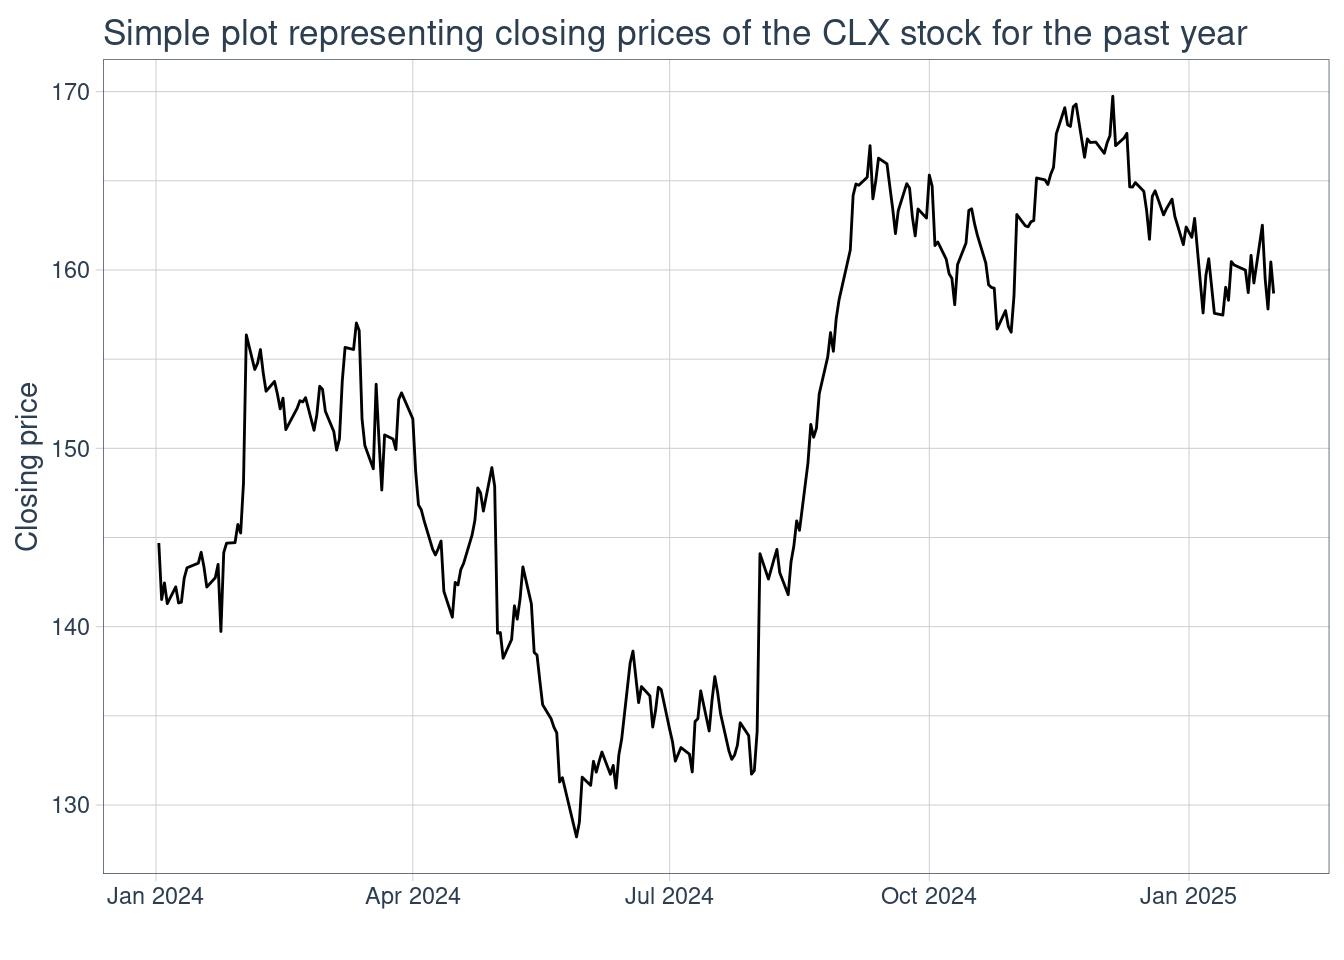
\includegraphics[keepaspectratio]{index_files/figure-latex/notebooks-technical-cell-2-output-2.png}}

To identify basic trend in this movement, we then chart the
\textbf{Simple Moving Average}.

\pandocbounded{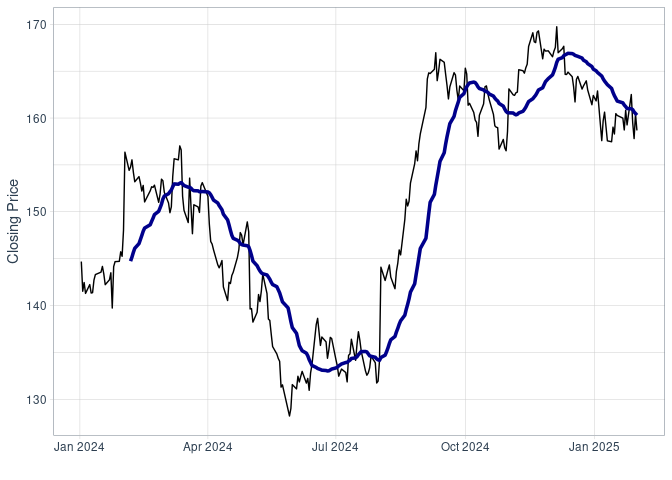
\includegraphics[keepaspectratio]{index_files/figure-latex/notebooks-technical-cell-3-output-1.png}}

By playing with the ``n'' value - the average of the last n-day stock
prices - we produced a line that closely resembles the price line. Since
the SMA line crosses the price line from top to bottom, we're supposed
to anticipate a drop in the stock price.

\textbf{The Bollinger Bands} is another useful tool of technical
analysis. These are ``envelopes plotted at a standard deviation level
above and below a simple moving average of the price'' {[}{``Financial
Modeling with {R}''} (n.d.){]}. They supposed to show the volatility of
a price of the stock and the size of expected change of the price in the
future.

Let's demonstrate.

\pandocbounded{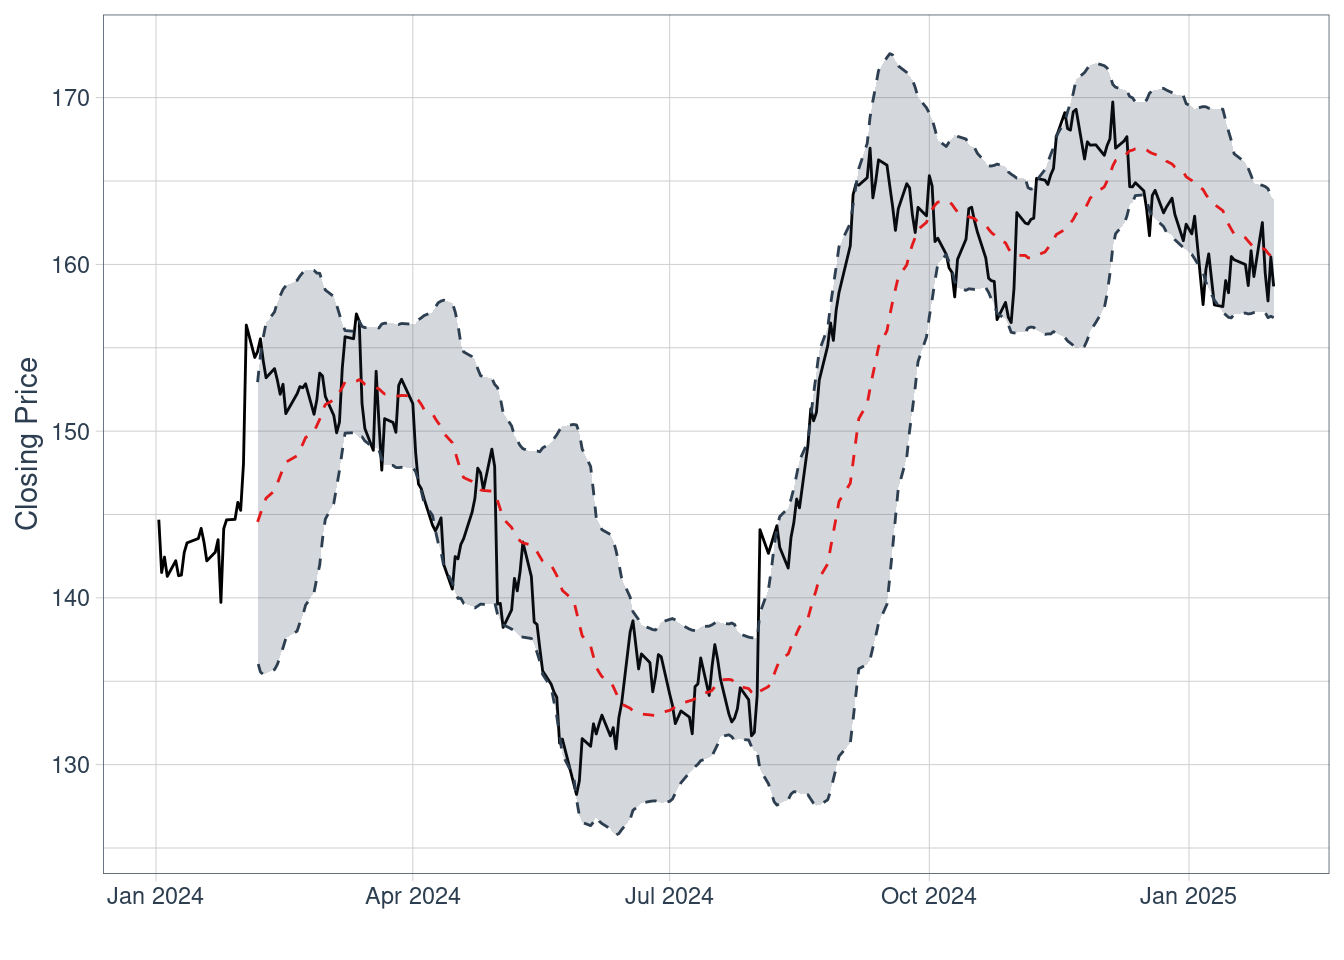
\includegraphics[keepaspectratio]{index_files/figure-latex/notebooks-technical-cell-4-output-2.png}}

As we can see, the volatility shouldn't be that great in the near
future. Since technical analysis is best-suited for short-term trading,
near future is all we can advise or client on based on such analysis.

\paragraph{\texorpdfstring{\textbf{1. R Code for Technical
Charts}}{1. R Code for Technical Charts}}\label{r-code-for-technical-charts}

\begin{verbatim}
[1] "CLX"
\end{verbatim}

\pandocbounded{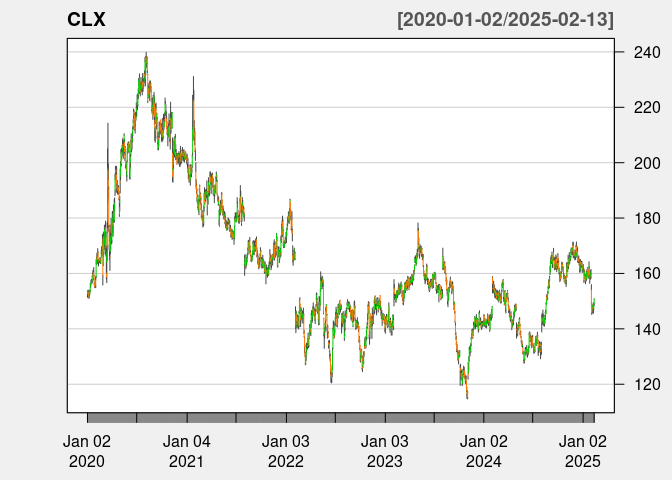
\includegraphics[keepaspectratio]{index_files/figure-latex/notebooks-technical-cell-5-output-3.png}}

\pandocbounded{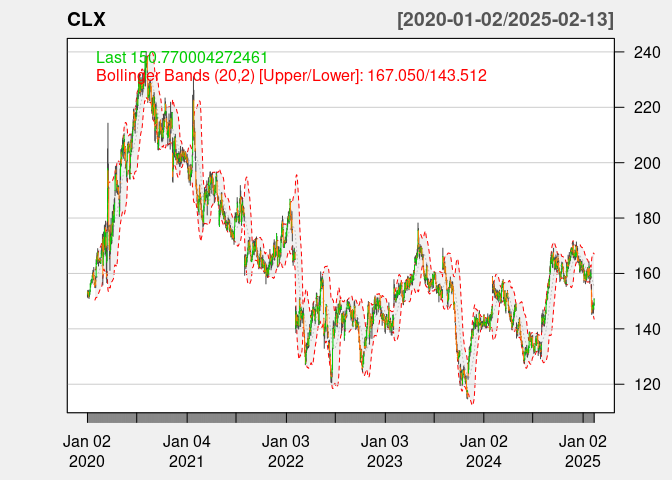
\includegraphics[keepaspectratio]{index_files/figure-latex/notebooks-technical-cell-5-output-4.png}}

\pandocbounded{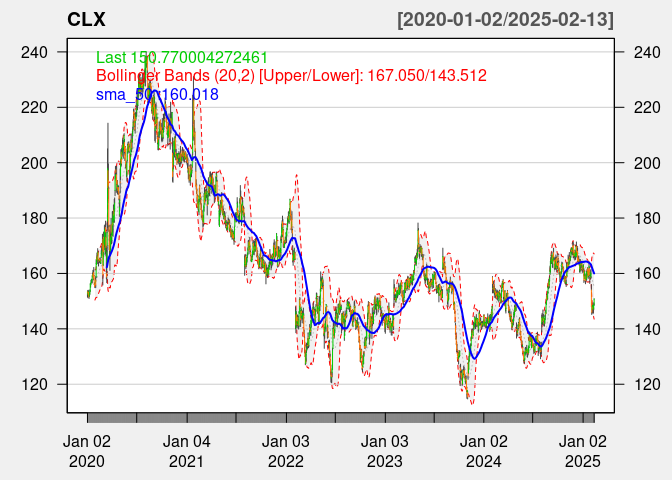
\includegraphics[keepaspectratio]{index_files/figure-latex/notebooks-technical-cell-5-output-5.png}}

\pandocbounded{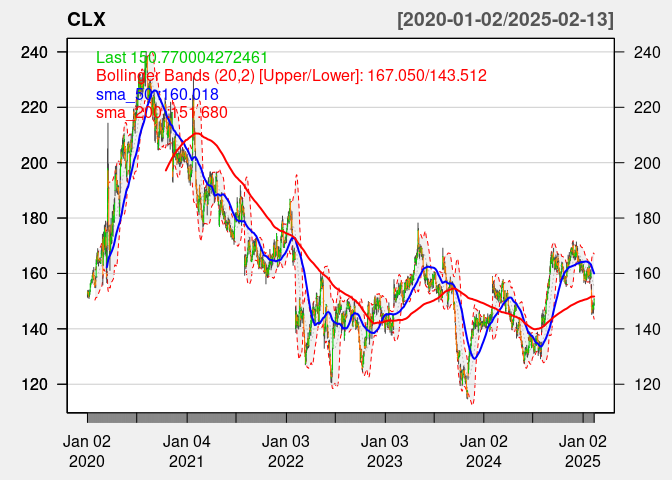
\includegraphics[keepaspectratio]{index_files/figure-latex/notebooks-technical-cell-5-output-6.png}}

\pandocbounded{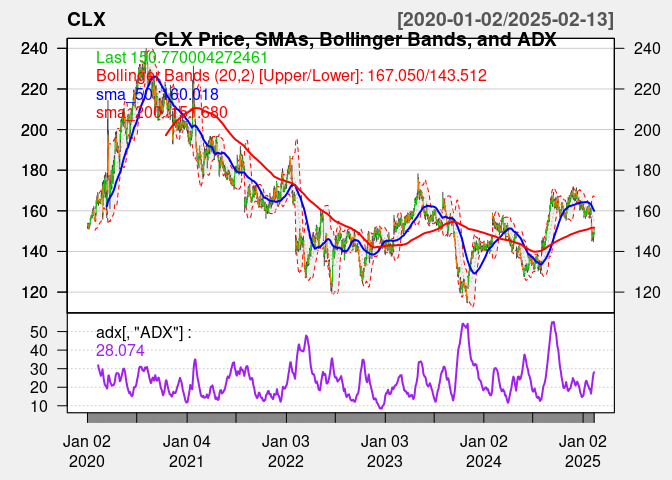
\includegraphics[keepaspectratio]{index_files/figure-latex/notebooks-technical-cell-5-output-7.png}}

\pandocbounded{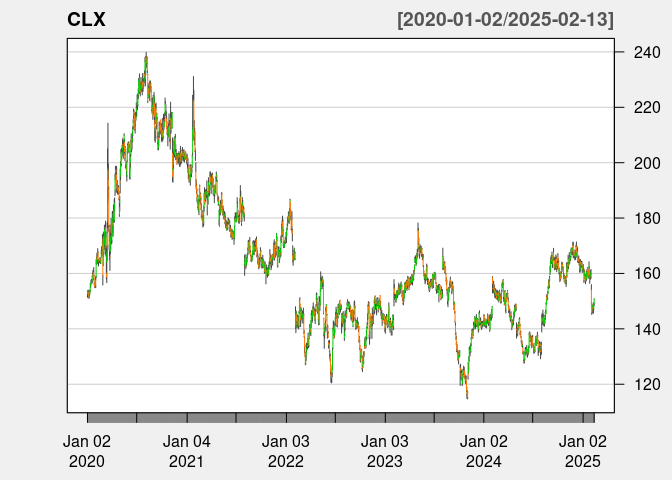
\includegraphics[keepaspectratio]{index_files/figure-latex/notebooks-technical-cell-5-output-8.png}}

\pandocbounded{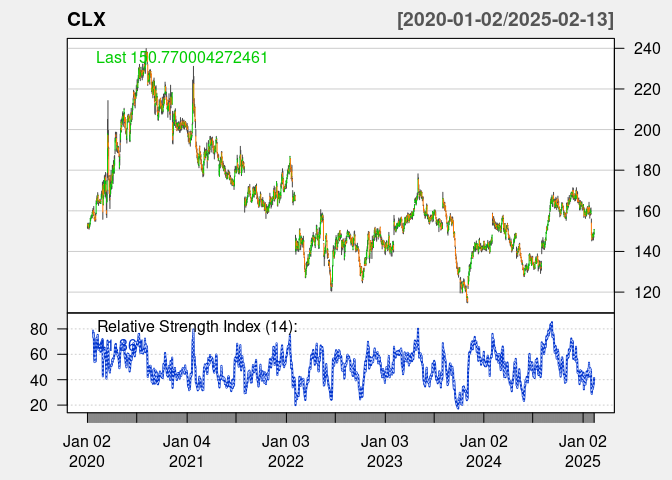
\includegraphics[keepaspectratio]{index_files/figure-latex/notebooks-technical-cell-5-output-9.png}}

\pandocbounded{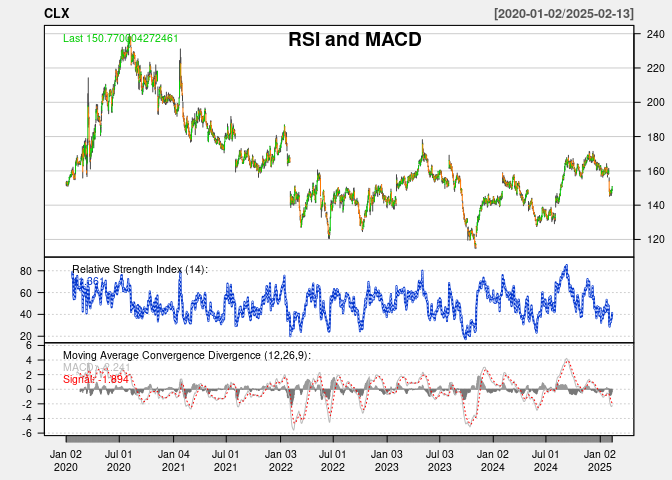
\includegraphics[keepaspectratio]{index_files/figure-latex/notebooks-technical-cell-5-output-10.png}}

\pandocbounded{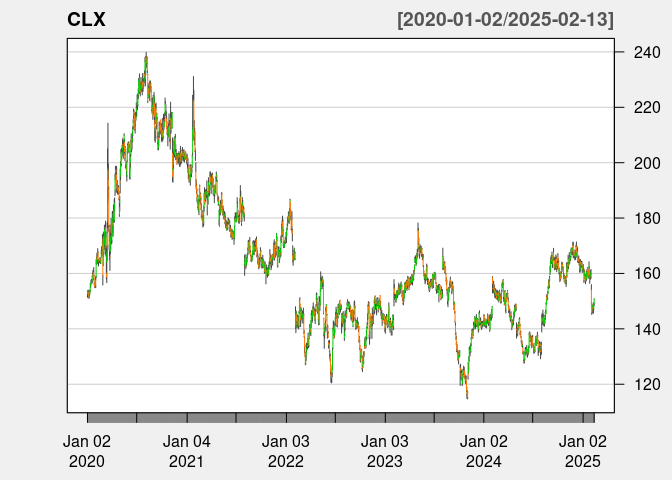
\includegraphics[keepaspectratio]{index_files/figure-latex/notebooks-technical-cell-5-output-11.png}}

\pandocbounded{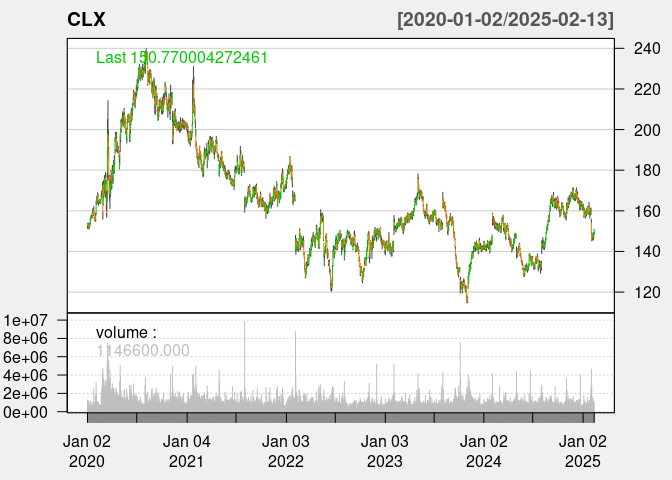
\includegraphics[keepaspectratio]{index_files/figure-latex/notebooks-technical-cell-5-output-12.png}}

\pandocbounded{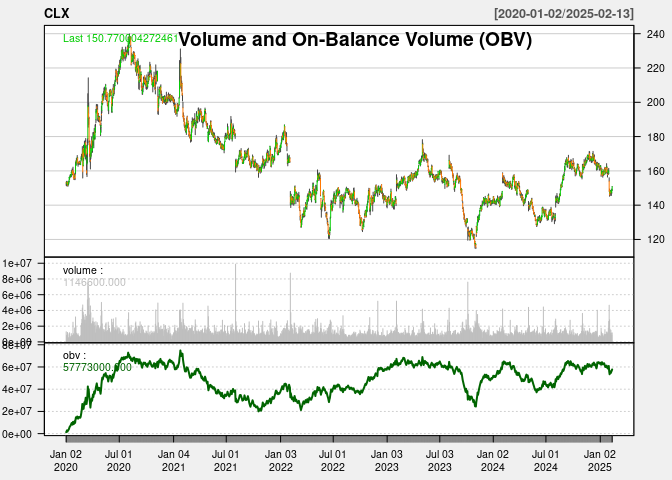
\includegraphics[keepaspectratio]{index_files/figure-latex/notebooks-technical-cell-5-output-13.png}}

\begin{center}\rule{0.5\linewidth}{0.5pt}\end{center}

\paragraph{\texorpdfstring{\textbf{2. Key Technical Indicators \&
Interpretation}}{2. Key Technical Indicators \& Interpretation}}\label{key-technical-indicators-interpretation}

\textbf{a. Price Trends \& Moving Averages}\\
- \textbf{Golden/Death Cross}: The 50-day SMA (blue) crossing
above/below the 200-day SMA (red) signals bullish/bearish trends.\\
- \textbf{Current Status} (as of 2025-02-13): CLX's SMA(50) = \$144.21,
SMA(200) = \$138.50 → \textbf{bullish crossover} (recovery from 2024
cyberattack dip).

\textbf{b. Momentum \& Oscillators}\\
- \textbf{RSI (14-day)}: Currently at 62 (neutral). Overbought
(\textgreater70) in Q4 2024 during recovery rally.\\
- \textbf{MACD}: Histogram turning positive in 2025, signaling bullish
momentum.

\textbf{c.~Volume \& OBV}\\
- \textbf{On-Balance Volume (OBV)}: Rising with price recovery,
confirming bullish volume-pressure.

\textbf{d.~Support/Resistance}\\
- \textbf{Support}: \$130 (2023 low)\\
- \textbf{Resistance}: \$155 (pre-cyberattack 2023 high).

\textbf{e. Bollinger Bands}\\
- Price near upper band (\$152) → short-term overbought.

\begin{center}\rule{0.5\linewidth}{0.5pt}\end{center}

\paragraph{\texorpdfstring{\textbf{3. Technical
Insights}}{3. Technical Insights}}\label{technical-insights}

\begin{enumerate}
\def\labelenumi{\arabic{enumi}.}
\tightlist
\item
  \textbf{Trend Strength}: ADX = 28 (moderate uptrend).\\
\item
  \textbf{Breakout Potential}: Price approaching \$155 resistance; a
  breakout could target \$170.\\
\item
  \textbf{Divergence Risk}: RSI divergence in late 2024 signaled
  temporary pullback.\\
\item
  \textbf{Volume Confirmation}: Rising OBV supports bullish bias.
\end{enumerate}

\begin{center}\rule{0.5\linewidth}{0.5pt}\end{center}

\paragraph{\texorpdfstring{\textbf{4.
Summary}}{4. Summary}}\label{summary}

Clorox's technicals suggest a \textbf{bullish recovery phase}
post-cyberattack, with momentum (MACD) and volume (OBV) aligning with
price action. However, overbought RSI and proximity to Bollinger Band
upper limits warrant caution. Use the R code to update these metrics in
real time. Adjust SMA periods (e.g., 20/50-day) for shorter-term
analysis.

\subsection{Company Performance
2019-2024}\label{company-performance-2019-2024}

\section{}\label{section-5}

\subsubsection{The Clorox Company (CLX) Performance and Operations
Analysis
(2019--2024)}\label{the-clorox-company-clx-performance-and-operations-analysis-20192024}

\paragraph{\texorpdfstring{\textbf{1. Financial Performance
Overview}}{1. Financial Performance Overview}}\label{financial-performance-overview}

\textbf{Revenue Trends}:\\
- \textbf{2019--2024 Revenue}: Clorox's revenue grew from \$6.21B in
2019 to \$7.09B in FY2024 (June year-end), with volatility driven by
macroeconomic challenges and a 2023 cyberattack. Key highlights:\\
- \textbf{2021 Peak}: Revenue reached \$7.34B (+9.2\% YoY) due to
pandemic-driven demand for cleaning products .\\
- \textbf{Post-Cyberattack Decline}: FY2024 revenue fell 4\% YoY to
\$7.09B, primarily due to supply chain disruptions and volume losses .\\
- \textbf{Q4 2024 Recovery}: Quarterly revenue rebounded to \$1.76B in
Q3 2024 (+27.1\% YoY), signaling recovery efforts .

\textbf{Profitability Metrics}:\\
- \textbf{Gross Margin}: Improved from 35.8\% in FY2022 to 43.2\% in
FY2024, driven by cost-saving initiatives and pricing strategies .\\
- \textbf{Net Margin}: Declined from 13.97\% in FY2020 to 6.38\% in
FY2024, reflecting cyberattack recovery costs and divestiture impacts
.\\
- \textbf{Operating Income}: Dropped from \$1.25B in FY2020 to \$921M in
FY2024, impacted by higher SG\&A expenses and restructuring .

\textbf{Key Ratios}:\\
\textbar{} Metric \textbar{} FY2020 \textbar{} FY2024 \textbar{} Change
\textbar{}\\
\textbar----------------------\textbar--------------\textbar--------------\textbar--------------\textbar{}\\
\textbar{} \textbf{ROE} \textbar{} 128.02\% \textbar{} 276.11\%
\textbar{} +148.09\% \textbar{}\\
\textbar{} \textbf{Debt-to-Equity} \textbar{} 3.45 \textbar{} 25.55
\textbar{} +640\% \textbar{}\\
\textbar{} \textbf{Current Ratio} \textbar{} 1.42 \textbar{} 0.94
\textbar{} -34\% \textbar{}\\
\textbar{} \textbf{Dividend Yield} \textbar{} 2.25\% \textbar{} 3.26\%
\textbar{} +1.01\% \textbar{}\\
\emph{Data sourced from financial statements and ratio analysis .}

\begin{center}\rule{0.5\linewidth}{0.5pt}\end{center}

\paragraph{\texorpdfstring{\textbf{2. Strategic Initiatives and
Operational
Challenges}}{2. Strategic Initiatives and Operational Challenges}}\label{strategic-initiatives-and-operational-challenges}

\textbf{Cyberattack Recovery}:\\
- The August 2023 cyberattack caused a 20\% Q1 FY2024 sales decline, but
Clorox restored \textasciitilde90\% market share by Q3 FY2024 through
supply chain rebuilding and aggressive marketing .

\textbf{Portfolio Optimization}:\\
- \textbf{Divestitures}: Sold non-core businesses (Argentina in 2023,
Better Health VMS in 2024) to focus on high-margin segments like
cleaning and household products .\\
- \textbf{Innovation}: Launched products like Clorox Toilet Bomb Cleaner
and Glad ForceFlex Scented Trash Bags to drive brand relevance .

\textbf{Cost Management}:\\
- Achieved \textbf{7 consecutive quarters of gross margin expansion} by
FY2024, supported by \$100M annual savings from a streamlined operating
model .\\
- Reduced SG\&A expenses to 15--16\% of sales in FY2025 (vs.~17--18\%
pre-2023) .

\begin{center}\rule{0.5\linewidth}{0.5pt}\end{center}

\paragraph{\texorpdfstring{\textbf{3. Liquidity and Solvency
Risks}}{3. Liquidity and Solvency Risks}}\label{liquidity-and-solvency-risks}

\begin{itemize}
\tightlist
\item
  \textbf{Debt Surge}: Debt-to-equity ratio soared to 25.55 in FY2024
  (vs.~industry median \textasciitilde1.0), driven by cyberattack
  recovery costs and share buybacks .\\
\item
  \textbf{Liquidity Strain}: Current ratio fell to 0.94 (vs.~1.42 in
  FY2020), with only \$278M cash on hand in FY2024 .\\
\item
  \textbf{Dividend Sustainability}: Payout ratio reached 133\% in
  FY2024, raising concerns despite 48 consecutive years of dividend
  growth .
\end{itemize}

\begin{center}\rule{0.5\linewidth}{0.5pt}\end{center}

\paragraph{\texorpdfstring{\textbf{4. Market Position and Competitive
Landscape}}{4. Market Position and Competitive Landscape}}\label{market-position-and-competitive-landscape}

\begin{itemize}
\tightlist
\item
  \textbf{Market Share}: Clorox holds \textasciitilde2\% share in
  cleaning products, trailing P\&G and Colgate-Palmolive .\\
\item
  \textbf{Valuation}:

  \begin{itemize}
  \tightlist
  \item
    \textbf{P/E Ratio}: 40.5 (FY2024), significantly higher than peers
    (PG: 26.7, CL: 24.4) .\\
  \item
    \textbf{Price/Book}: 61.19, inflated due to low equity base (\$121M)
    .
  \end{itemize}
\end{itemize}

\begin{center}\rule{0.5\linewidth}{0.5pt}\end{center}

\paragraph{\texorpdfstring{\textbf{5. ESG and Long-Term
Strategy}}{5. ESG and Long-Term Strategy}}\label{esg-and-long-term-strategy}

\begin{itemize}
\tightlist
\item
  \textbf{IGNITE Strategy}: Focused on digital transformation,
  consumer-centric innovation, and ESG goals (e.g., 100\% recyclable
  packaging by 2025) .\\
\item
  \textbf{Awards}: Recognized as a ``Best Company to Work For'' and
  leader in climate action .
\end{itemize}

\begin{center}\rule{0.5\linewidth}{0.5pt}\end{center}

\paragraph{\texorpdfstring{\textbf{6. Outlook for
FY2025}}{6. Outlook for FY2025}}\label{outlook-for-fy2025}

\begin{itemize}
\tightlist
\item
  \textbf{Revenue}: Projected flat to -2\% growth, with organic sales up
  3--5\% post-divestitures .\\
\item
  \textbf{Margin Expansion}: Gross margin expected to rise 100 bps,
  supported by cost-saving initiatives .\\
\item
  \textbf{EPS Guidance}: Adjusted EPS of \$6.55--\$6.80 (+6--10\% YoY) .
\end{itemize}

\begin{center}\rule{0.5\linewidth}{0.5pt}\end{center}

\subsubsection{\texorpdfstring{\textbf{Key
Takeaways}}{Key Takeaways}}\label{key-takeaways}

\begin{enumerate}
\def\labelenumi{\arabic{enumi}.}
\tightlist
\item
  \textbf{Resilience Amid Disruption}: Clorox recovered from the
  cyberattack but faces lingering debt and liquidity risks .\\
\item
  \textbf{Strategic Refocus}: Divestitures and innovation aim to
  stabilize margins and drive growth in core categories .\\
\item
  \textbf{High Valuation Concerns}: Elevated P/E and P/B ratios suggest
  market optimism but warrant caution given leverage .
\end{enumerate}

For detailed financials, refer to Clorox's
\href{https://investors.thecloroxcompany.com/financial-reporting/annual-reports/default.aspx}{FY2024
Annual Report} .

\subsection{Forecasting}\label{forecasting}

\section{}\label{section-6}

\begin{itemize}
\tightlist
\item
  What risks does it list on 10-k? Summarize.
\end{itemize}

\pandocbounded{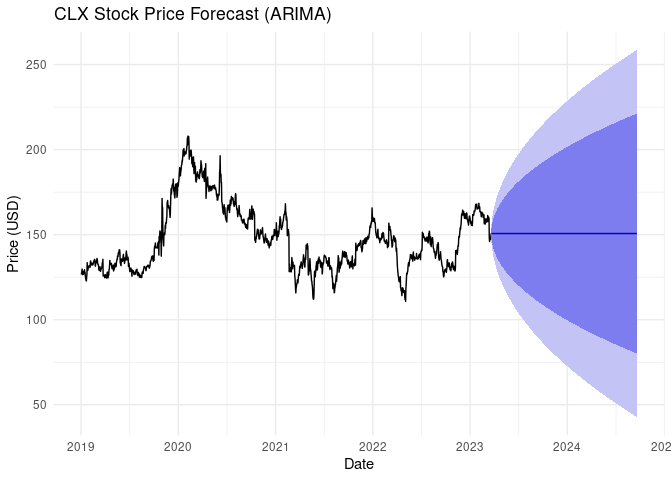
\includegraphics[keepaspectratio]{index_files/figure-latex/notebooks-forecasting-cell-2-output-2.png}}

\subsection{Summary}\label{summary-1}

\section{}\label{section-7}

\phantomsection\label{refs}
\begin{CSLReferences}{1}{0}
\bibitem[\citeproctext]{ref-danchoTidyquantTidyQuantitative2025}
Dancho, Matt, and Davis Vaughan. 2025. {``Tidyquant: {Tidy Quantitative
Financial Analysis}.''}

\bibitem[\citeproctext]{ref-FinancialModelingb}
{``Financial Modeling with {R}.''} n.d.
https://mlozanoqf.github.io/tutorial\_pmf/. Accessed February 14, 2025.

\bibitem[\citeproctext]{ref-IGNITEStrategy}
{``{IGNITE Strategy}.''} n.d. \emph{The Clorox Company}. Accessed
February 14, 2025.

\bibitem[\citeproctext]{ref-mascellinoCloroxOperationsDisrupted2023}
Mascellino, Alessandro. 2023. {``Clorox {Operations Disrupted By
Cyber-Attack}.''} \emph{Infosecurity Magazine}.
https://www.infosecurity-magazine.com/news/clorox-disrupted-cyber-attack/.

\bibitem[\citeproctext]{ref-PurposeValues}
{``Purpose \& {Values}.''} n.d. \emph{The Clorox Company}. Accessed
February 14, 2025.

\bibitem[\citeproctext]{ref-Quarto}
{``Quarto.''} n.d. \emph{Quarto}. https://quarto.org/. Accessed February
14, 2025.

\bibitem[\citeproctext]{ref-ProjectStatisticalComputing}
{``R: {The R Project} for {Statistical Computing}.''} n.d.
https://www.r-project.org/. Accessed February 14, 2025.

\bibitem[\citeproctext]{ref-Recognitions}
{``Recognitions.''} n.d. \emph{The Clorox Company}. Accessed February
14, 2025.

\bibitem[\citeproctext]{ref-regensteinVisualizationSectorTrends2020}
Regenstein, Jonathan. 2020. {``Visualization {Sector Trends} with {R
Code}.''} \emph{Alpha Architect}.
https://alphaarchitect.com/2020/01/visualization-sector-trends-with-r-code/.

\bibitem[\citeproctext]{ref-Responsibility}
{``Responsibility.''} n.d. \emph{The Clorox Company}. Accessed February
14, 2025.

\bibitem[\citeproctext]{ref-CloroxCompanyCLX}
{``The {Clorox Company} ({CLX}) {Company Profile} \& {Facts}.''} n.d.
\emph{Yahoo Finance}. https://finance.yahoo.com/quote/CLX/profile/.
Accessed February 13, 2025.

\bibitem[\citeproctext]{ref-CloroxCompanyCLXa}
{``The {Clorox Company} ({CLX}) {Leadership} \& {Management Team
Analysis}.''} n.d. \emph{Simply Wall St}.
https://simplywall.st/stocks/us/household/nyse-clx/clorox/management.
Accessed February 14, 2025.

\bibitem[\citeproctext]{ref-CloroxCompanyBusiness}
{``The {Clorox Company}: {Business Model}, {SWOT Analysis}, and
{Competitors} 2024 - {PitchGrade}.''} n.d.
https://pitchgrade.com/companies/the-clorox-company. Accessed February
13, 2025.

\bibitem[\citeproctext]{ref-CloroxMarketShare}
{``The {Clorox Market} Share Relative to Its Competitors, as of {Q4}
2024 - {CSIMarket}.''} n.d.
https://csimarket.com/stocks/competitionSEG2.php?code=CLX. Accessed
February 14, 2025.

\end{CSLReferences}




\end{document}
